\documentclass[11pt,a4paper]{article}
% Společné nastavení pro protokoly KI/PZS (pdfLaTeX, Overleaf výchozí kompilátor)
\usepackage[utf8]{inputenc}
\usepackage[T1]{fontenc}
\usepackage[czech]{babel}
\usepackage{lmodern}
\usepackage{amsmath}
\usepackage[a4paper,margin=2.5cm]{geometry}
\usepackage{microtype}
\usepackage{graphicx}
\usepackage{booktabs}
\usepackage{array}
\usepackage{tabularx}
\usepackage{xcolor}
\usepackage{enumitem}
\usepackage[font=small,labelfont=bf]{caption}
\usepackage{subcaption}
\usepackage{float}
\usepackage{tikz}
\usetikzlibrary{arrows.meta,positioning,shapes.geometric,calc}
\usepackage{pgfplots}
\pgfplotsset{compat=1.17}
\usepackage[hidelinks]{hyperref}

\setlist{itemsep=2pt,topsep=4pt}
\setlength{\parindent}{0pt}
\setlength{\parskip}{6pt}

% Záporné znaménko v textových tabulkách: \m0,5 -> −0,5
\newcommand{\m}{$-$}

% Červená značka pro místa, která je třeba před odevzdáním doplnit
\newcommand{\doplnit}[1]{\textcolor{red}{\textbf{[DOPLNIT: #1]}}}

% Obrázek, který se zobrazí, jakmile je soubor nahrán; do té doby červený zástupce
\newcommand{\obrazekNeboZastupce}[3]{%
  \IfFileExists{#1}{\includegraphics[width=#2]{#1}}{%
    \fbox{\parbox[c][4cm][c]{\dimexpr#2-2\fboxsep-2\fboxrule\relax}{\centering\doplnit{#3}}}}}

% Styl vývojových diagramů
\tikzset{
  krok/.style={draw, rounded corners=3pt, minimum width=3.3cm, minimum height=1.15cm,
               align=center, font=\small, line width=0.5pt, draw=black!60},
  hlavni/.style={krok, draw=blue!70!black, fill=blue!8, line width=0.9pt},
  rozhodnuti/.style={draw, diamond, aspect=2.4, align=center, font=\small,
               inner sep=1pt, line width=0.5pt, draw=black!60},
  sipka/.style={-{Stealth[length=2.6mm]}, line width=0.5pt, draw=black!60},
  popisek/.style={font=\footnotesize, text=black!70}
}


\addto\captionsczech{\renewcommand{\refname}{Literatura}}

\title{\textbf{Seminární práce II}\\[2pt]
       Klasifikace hlasu /a/ v databázi VOICED}
\author{Jakub Jančařík, Matěj Bureš, Robert Thomas Seaborn}
\date{Předmět: Počítačové zpracování signálu (KI/PZS)\\[2pt] 15.~2.~2026}

\begin{document}
\maketitle

%==============================================================================
\section{Zadání}
%==============================================================================
Cílem je klasifikovat 208 nahrávek samohlásky /a/ z databáze VOICED \cite{voiced,physionet}
na zdravé a patologické hlasy a u patologických určit typ poruchy. Úspěšnost se porovnává
s diagnózami expertů uvedenými v hlavičkových souborech.

\begin{itemize}
  \item \textbf{Fáze 1:} zdravý $\times$ patologický hlas.
  \item \textbf{Fáze 2:} typ poruchy u patologických nahrávek (hyperkinetická dysfonie,
        hypokinetická dysfonie, reflux laryngitis).
  \item \textbf{Příznaky:} základní frekvence F0, jitter, shimmer, HNR, spektrální a kepstrální
        příznaky včetně MFCC, všechny počítané vlastními algoritmy. Knihovna WFDB slouží jen ke
        čtení signálů a diagnóz z hlaviček.
  \item \textbf{Hodnocení:} matice záměn, úspěšnost po skupinách a vizualizace v prostoru příznaků.
\end{itemize}

Použitý software: Python, \texttt{numpy}, \texttt{scipy} \cite{scipy}, \texttt{pandas},
\texttt{matplotlib} a \texttt{scikit-learn} \cite{sklearn} (jen klasifikátory, standardizace a
křížová validace). Zdrojové kódy tvoří programovou část práce.

%==============================================================================
\section{Data a příznaky}
%==============================================================================
Databáze obsahuje 208 nahrávek (vzorkovací frekvence 8~kHz), diagnóza je v komentářích hlavičky
každého záznamu. Podle hlaviček je v souboru 57 zdravých a 151 patologických hlasů (zadání uvádí
58 a 150). Patologické nahrávky tvoří tři skupiny: hyperkinetická dysfonie (73), hypokinetická
dysfonie (40) a reflux laryngitis (38). U nahrávky voice143 je v anotaci překlep
(„hyperkineti dysphonia“), který skript opraví.

Každá nahrávka se nejdříve zbaví offsetu, ořízne se na stabilní úsek (energetický práh 10~\%
maxima RMS v oknech 20~ms, bez prvních a posledních 0,2~s) a normalizuje se na amplitudu~1.
Z každé nahrávky vzniká 45 příznaků (tab.~\ref{tab:priznaky}).

\begin{table}[H]
\centering\small
\caption{Příznaky počítané z jedné nahrávky.}
\label{tab:priznaky}
\begin{tabularx}{\textwidth}{>{\raggedright\arraybackslash}p{2.7cm}>{\raggedright\arraybackslash}X r >{\raggedright\arraybackslash}p{5.3cm}}
\toprule
Skupina & Příznaky & Počet & Metoda\\
\midrule
Základní frekvence & medián a směrodatná odchylka F0, podíl znělých rámců & 3 &
  normovaná autokorelace, rámce 40~ms (krok 20~ms), rozsah 70--400~Hz, první vrchol s výškou
  alespoň 90~\% maxima, parabolická interpolace píku\\
Poměr harmonických a šumu & HNR (průměr, směrodatná odchylka) & 2 &
  z výšky autokorelačního píku $r$, vztah \eqref{eq:hnr} \cite{boersma}\\
Perturbace & jitter local, jitter RAP, shimmer local, shimmer APQ3 & 4 &
  z jednotlivých period hlasivek (vrcholy upřesněné parabolou)\\
Časové & míra průchodů nulou (ZCR) & 1 & průměrný počet průchodů nulou\\
Spektrální (FFT) & těžiště, rozptyl, roll-off 85~\%, plochost, energie ve 4 pásmech, poměr nízké a vysoké energie & 9 &
  průměrné výkonové spektrum (Hannovo okno, 512 vzorků, krok 256)\\
Kepstrální & CPP (průměr, směrodatná odchylka) & 2 &
  reálné kepstrum z log. spektra, výška píku nad regresní přímkou \cite{hillenbrand}\\
MFCC & 12 koeficientů (průměr a směrodatná odchylka) & 24 &
  pre-emfáze 0,97, rámce 32~ms, 26 melovských filtrů, DCT, bez $c_0$ \cite{davis}\\
\bottomrule
\end{tabularx}
\end{table}

\begin{equation}
  \mathrm{HNR} = 10\log_{10}\frac{r}{1-r}\ \text{[dB]},
  \label{eq:hnr}
\end{equation}
kde $r$ je normovaná výška autokorelačního píku na zpoždění odpovídajícím periodě F0.

Perioda se neurčuje prostým maximem autokorelace. U periodického signálu má autokorelace téměř
stejně vysoký vrchol i na dvojnásobku periody a korekce vlivem okna \cite{boersma} dlouhá zpoždění
ještě zesiluje, takže maximum často padne na $2T$ a F0 vyjde o oktávu níž. Bere se proto první
vrchol, jehož výška dosahuje alespoň 90~\% maxima. Pohlaví z hlavičky slouží jen ke kontrole
věrohodnosti F0, klasifikátor ho nepoužívá. S prostým maximem vycházel u 62 ze 135 žen medián F0
pod 140~Hz, medián F0 žen jen 160~Hz a typická směrodatná odchylka F0 uvnitř jedné nahrávky 46~Hz
(skoky mezi $T$ a $2T$). Po úpravě je medián F0 206~Hz u žen a 144~Hz u mužů, pod 140~Hz zůstává
7 žen (všechny s patologickým hlasem) a typická směrodatná odchylka F0 v nahrávce klesla na 2,8~Hz.

Obrázek~\ref{fig:priklad} ukazuje zdravý a patologický hlas v čase, ve spektru a v kepstru.
Kepstrální pík odpovídá periodě základní frekvence (přibližně 7,7~ms, tedy 130~Hz u zdravého
a 8,5~ms, tedy 118~Hz u patologického hlasu).

\begin{figure}[H]
\centering
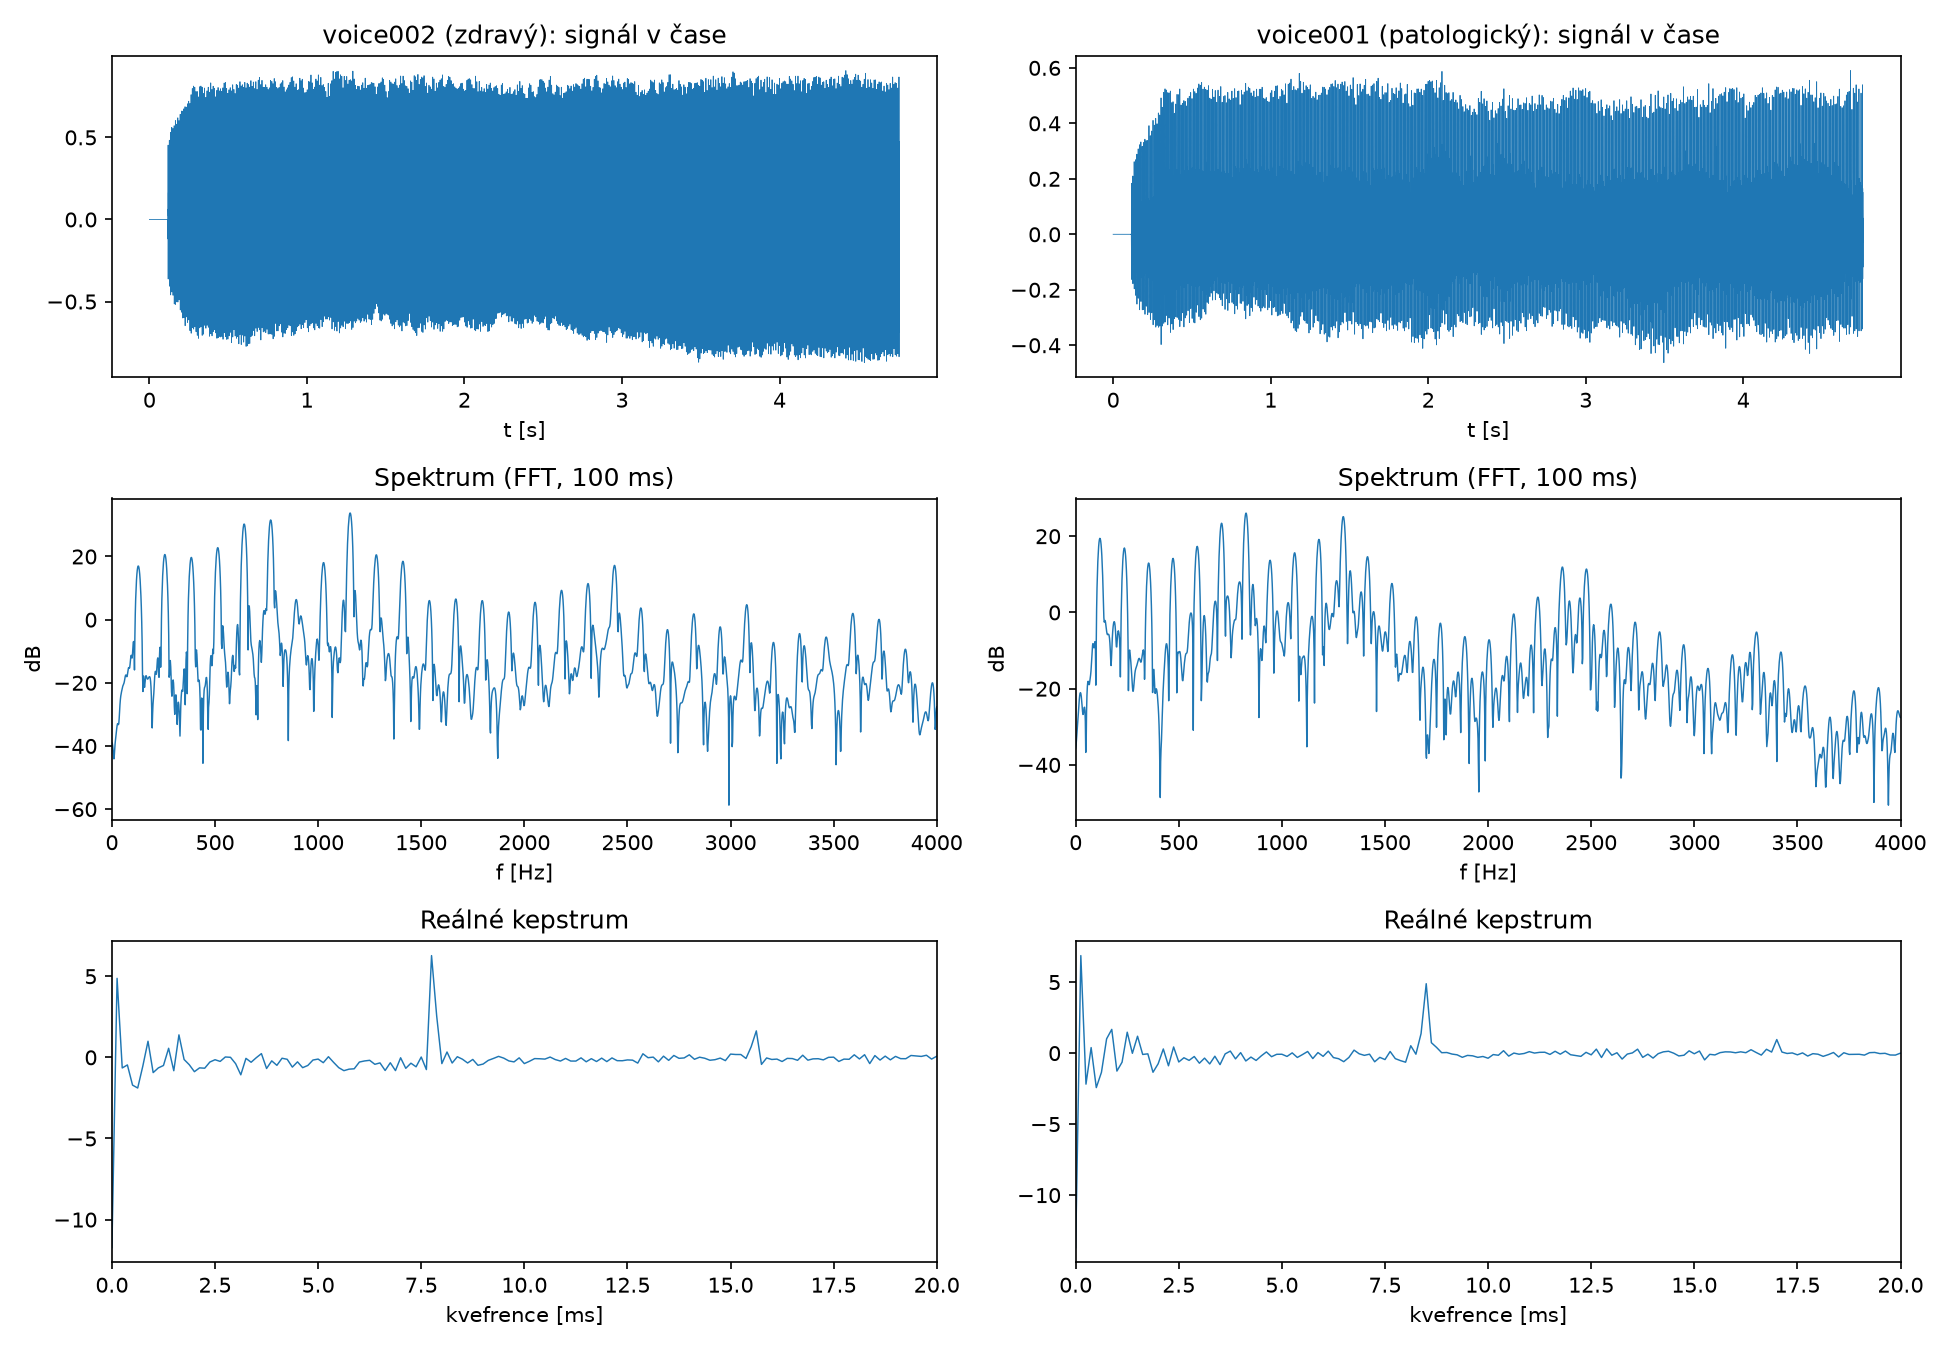
\includegraphics[width=0.95\textwidth]{figures/ukazka_signalu_spektra_kepstra.png}
\caption{Zdravý (voice002) a patologický (voice001) hlas: signál v čase, amplitudové spektrum (FFT,
100~ms) a reálné kepstrum.}
\label{fig:priklad}
\end{figure}

Obrázek~\ref{fig:box} ukazuje rozložení vybraných příznaků podle skupin. Hypokinetická dysfonie má
nejnižší HNR a CPP a nejvyšší shimmer a jitter (medián jitteru 2,5~\% oproti 0,6~\% u zdravých).
Reflux laryngitis je zdravému hlasu nejpodobnější, dokonce má nižší shimmer a vyšší CPP než zdraví.
Skupiny se ale uvnitř silně překrývají. Mediány všech příznaků po skupinách jsou v souboru
\texttt{mediany\_priznaku\_po\_skupinach.csv}.

\begin{figure}[H]
\centering
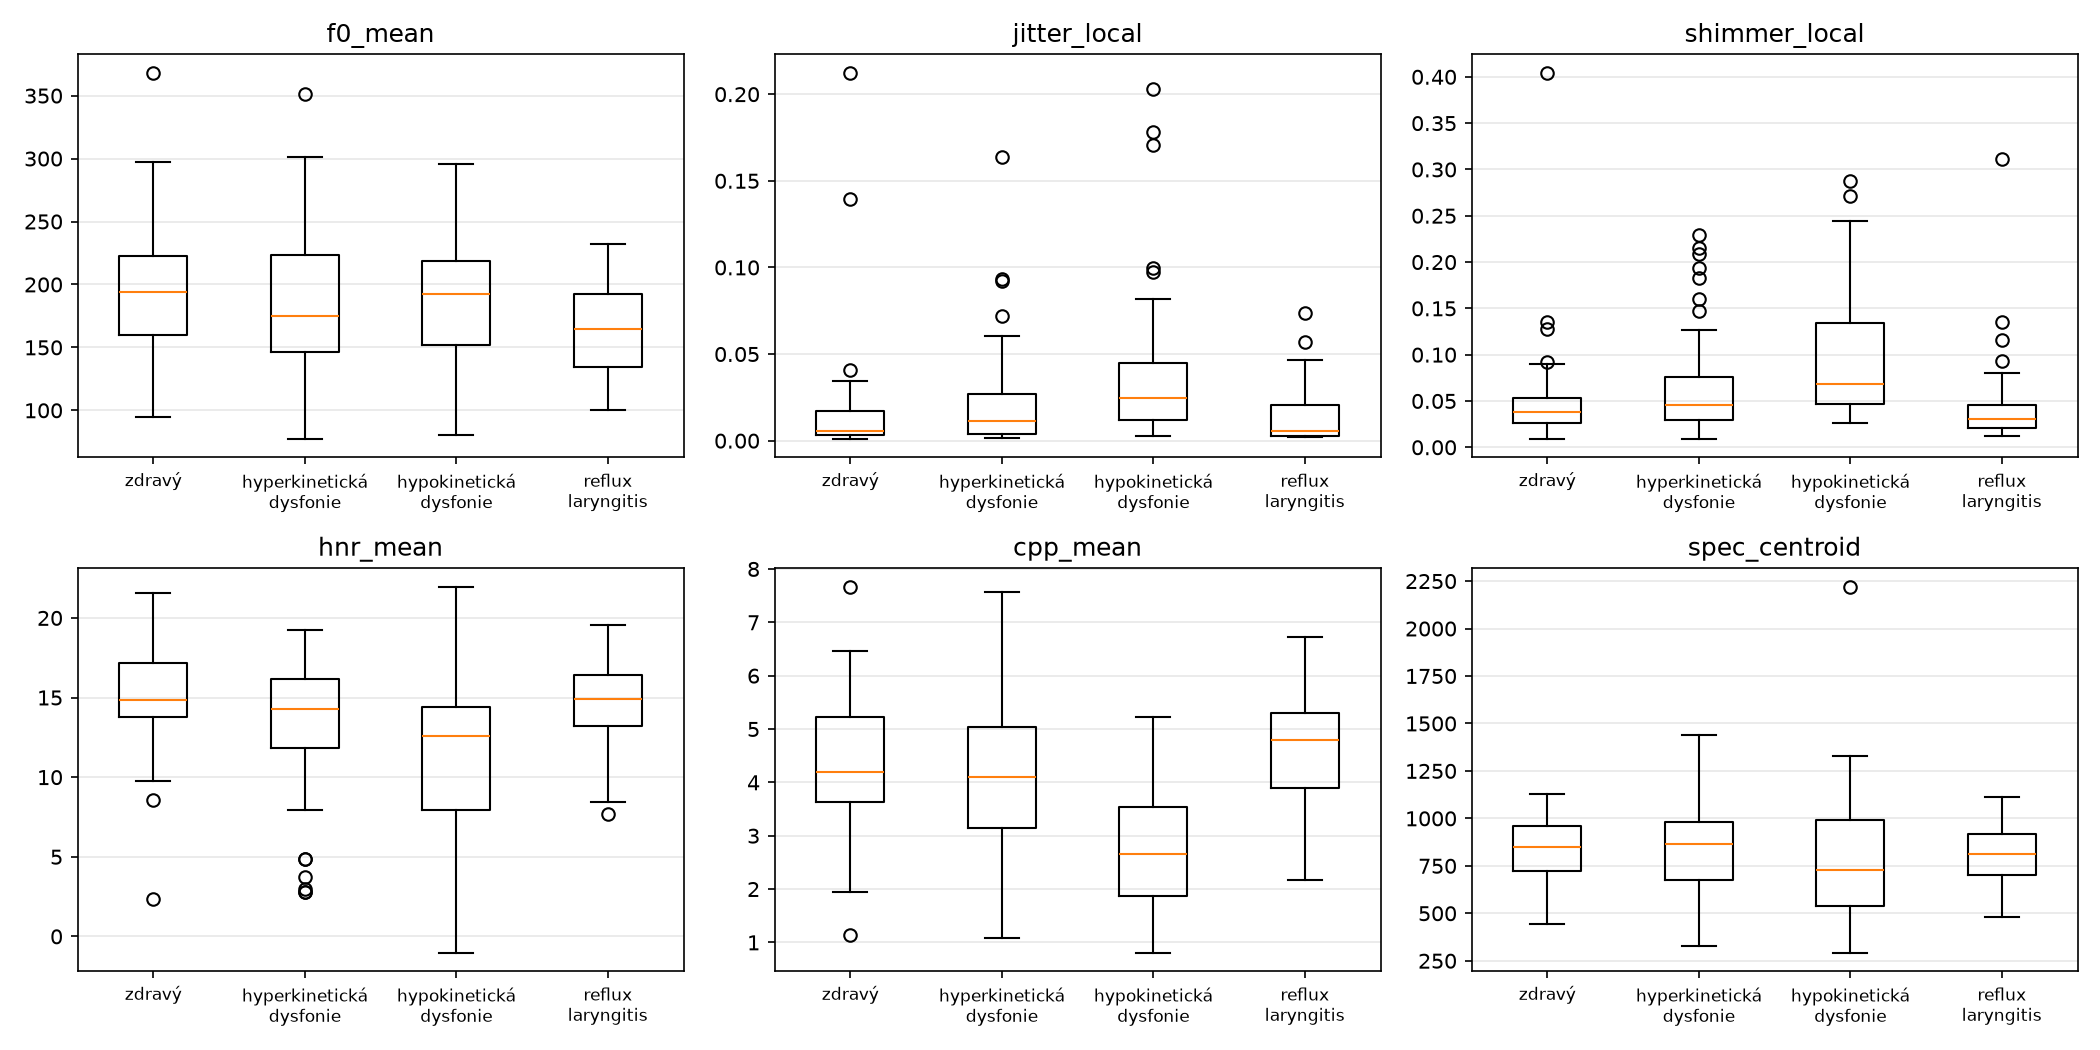
\includegraphics[width=\textwidth]{figures/boxploty_priznaku.png}
\caption{Rozložení vybraných příznaků podle skupin (medián, kvartily, odlehlé hodnoty).}
\label{fig:box}
\end{figure}

%==============================================================================
\section{Postup klasifikace}
%==============================================================================
Klasifikace běží ve dvou fázích a každá se hodnotí toutéž křížovou validací
(obr.~\ref{fig:diag-klas}).

\begin{figure}[H]
\centering
\begin{tikzpicture}
  \node[krok] (rec)  at (0,0)    {\textbf{Nahrávka /a/}\\{\footnotesize 208, 8 kHz}};
  \node[krok] (feat) at (4,0)    {\textbf{Příznaky}\\{\footnotesize 45, vlastní kód}};
  \node[krok] (std)  at (8,0)    {\textbf{Standardizace}\\{\footnotesize imputace mediánem}};
  \node[krok] (f1)   at (12,0)   {\textbf{Fáze 1}\\{\footnotesize SVM, zanořená CV}};
  \node[krok] (diag) at (0,-2.4) {\textbf{Diagnóza}\\{\footnotesize z hlavičky .hea}};
  \node[hlavni] (ev) at (4,-2.4) {\textbf{Hodnocení}\\{\footnotesize 5násobná CV (10$\times$), matice záměn}};
  \node[krok] (zdr)  at (8,-2.4) {\textbf{Zdravý}\\{\footnotesize bez 2. fáze}};
  \node[rozhodnuti] (dec) at (12,-2.4) {Patologický?};
  \node[krok] (f2)   at (12,-4.8) {\textbf{Fáze 2}\\{\footnotesize random forest}};
  \draw[sipka] (rec)--(feat);
  \draw[sipka] (feat)--(std);
  \draw[sipka] (std)--(f1);
  \draw[sipka] (rec)--(diag);
  \draw[sipka] (diag)--(ev);
  \draw[sipka] (f1)--(dec);
  \draw[sipka] (dec)--node[popisek,above]{ne}(zdr);
  \draw[sipka] (zdr)--(ev);
  \draw[sipka] (dec)--node[popisek,right]{ano}(f2);
  \draw[sipka] (f2.west) -| (ev.south);
\end{tikzpicture}
\caption{Vývojový diagram klasifikace: dvě fáze a porovnání s diagnózou.}
\label{fig:diag-klas}
\end{figure}

\begin{itemize}
  \item \textbf{Příprava:} chybějící hodnoty (2 nahrávky bez jitteru a shimmeru) se doplní mediánem
        a příznaky se standardizují (z-skóre), vždy jen podle trénovací části foldu.
  \item \textbf{Modely:} SVM s jádrem RBF, kNN (váhy podle vzdálenosti) a random forest (300 stromů).
        U SVM a lesa vyvažují třídy váhy. Hyperparametry se ladí zanořenou CV (viz níže).
  \item \textbf{Fáze 1 i fáze 2:} uvnitř každého foldu vnější CV probíhá 3násobná zanořená
        GridSearchCV na trénovací části: prohledává počet příznaků $k\in\{5,8,12,\text{vše}\}$
        (výběr F-statistikou ANOVA), $C\in\{1,3,10\}$ pro SVM a $k_{\text{sousedů}}\in\{3,5,7\}$
        pro kNN. Žádná informace z testovací části foldu tak neuniká do výběru příznaků ani
        do ladění hyperparametrů.
  \item \textbf{Fáze 2:} učí se jen na patologických nahrávkách, tři třídy. Skupiny s méně než
        10~nahrávkami by se sloučily do skupiny \emph{other}, v tomto souboru žádná taková není.
  \item \textbf{Kaskáda:} testovací nahrávka projde fází 1 a jen ta označená za patologickou fází 2.
        Pro každou fázi se bere model s nejvyšší průměrnou vyváženou přesností z opakované validace.
  \item \textbf{Validace:} stratifikovaná 5násobná křížová validace. Aby bylo vidět, nakolik výsledek
        závisí na náhodném rozdělení do foldů, opakuje se desetkrát s různým rozdělením a uvádí se
        průměr $\pm$ směrodatná odchylka. Matice záměn a tabulky po skupinách jsou z jednoho rozdělení
        (semínko 42). Hodnotí se přesnost, vyvážená přesnost, precision, recall, F1 a matice záměn.
\end{itemize}

%==============================================================================
\section{Výsledky}
%==============================================================================
Fáze 1 dosáhla vyvážené přesnosti $57{,}2 \pm 2{,}2$~\%, fáze 2 (typ poruchy) vyvážené přesnosti
$52{,}7 \pm 1{,}6$~\% (přesnost $50{,}3 \pm 1{,}8$~\%) a celá kaskáda se čtyřmi třídami přesnosti 36,1~\%.
Hodnoty $\pm$ jsou směrodatné odchylky přes 10 opakování křížové validace.

\subsection{Fáze 1: zdravý $\times$ patologický}
Tabulka~\ref{tab:faze1} porovnává modely ($k$ příznaků i hyperparametry laděny zanořenou CV).

\begin{table}[H]
\centering\small
\caption{Fáze 1: zdravý $\times$ patologický. Průměr $\pm$ směrodatná odchylka přes 10 opakování
5násobné křížové validace, v závorce jedno rozdělení se semínkem 42.}
\label{tab:faze1}
\begin{tabular}{lrr}
\toprule
Model & Přesnost [\%] & Vyvážená přesnost [\%]\\
\midrule
SVM (RBF)     & $55{,}3 \pm 2{,}0$ (52,4) & $\mathbf{57{,}2 \pm 2{,}2}$ (56,8)\\
kNN ($k=5$)   & $65{,}7 \pm 2{,}0$ (64,4) & $53{,}3 \pm 2{,}1$ (52,6)\\
Random forest & $64{,}6 \pm 3{,}0$ (58,7) & $56{,}5 \pm 3{,}1$ (51,3)\\
\bottomrule
\end{tabular}
\end{table}

Nejlepší SVM správně určil 38 z 57 zdravých (specificita 66,7~\%) a 71 ze 151 patologických
(senzitivita 47,0~\%). Triviální strategie „vždy patologický” má přesnost 72,6~\%, ale vyváženou
jen 50~\%, a proto je rozhodující vyvážená přesnost. kNN má nejvyšší přesnost (65,7~\%) jen proto,
že většinu nahrávek přiřadí k početnější patologické třídě. Jeho přesnost je přitom stále pod
triviální strategií a vyvážená přesnost 53,3~\% je blízko náhodě. Rozdíly mezi SVM a random
forestem (0,7 p.b.) jsou srovnatelné se směrodatnou odchylkou.

\subsection{Fáze 2: typ poruchy}
Tabulka~\ref{tab:faze2} platí pro 151 patologických nahrávek se třemi třídami.

\begin{table}[H]
\centering\small
\caption{Fáze 2: typ poruchy (jen patologické nahrávky). Průměr $\pm$ směrodatná odchylka přes
10 opakování, v závorce jedno rozdělení se semínkem 42.}
\label{tab:faze2}
\begin{tabular}{lrr}
\toprule
Model & Přesnost [\%] & Vyvážená přesnost [\%]\\
\midrule
SVM (RBF)     & $43{,}8 \pm 2{,}8$ (44,4) & $49{,}4 \pm 2{,}7$ (49,0)\\
kNN ($k=5$)   & $44{,}1 \pm 1{,}5$ (45,0) & $41{,}8 \pm 1{,}9$ (41,5)\\
Random forest & $50{,}3 \pm 1{,}8$ (51,0) & $\mathbf{52{,}7 \pm 1{,}6}$ (53,8)\\
\bottomrule
\end{tabular}
\end{table}

Náhodné hádání dává 33~\% vyváženě, strategie „vždy hyperkinetická“ 48,3~\% přesnosti a 33~\%
vyváženě. Random forest je v přesnosti jen mírně nad touto hranicí, ve vyvážené přesnosti
o 20 p.b. nad náhodou.

\subsection{Kaskáda}
Kaskáda používá SVM ve fázi 1 a random forest ve fázi 2 (tab.~\ref{tab:kaskada}, obr.~\ref{fig:matice}).
Celková přesnost je 36,1~\% (75 ze 208), triviální strategie dává 35,1~\%. Jako patologické bylo
označeno 55,6~\% skutečně patologických nahrávek (jiné rozdělení foldů než ve fázi 1, proto jiné
číslo než 47,0~\%).

\begin{table}[H]
\centering\small
\caption{Kaskáda: úspěšnost po skupinách.}
\label{tab:kaskada}
\begin{tabular}{lrrrr}
\toprule
Skupina & Počet & Precision [\%] & Úspěšnost (recall) [\%] & F1 [\%]\\
\midrule
zdravý                  & 57 & 35,6 & 64,9 & 46,0\\
hyperkinetická dysfonie & 73 & 27,9 & 16,4 & 20,7\\
hypokinetická dysfonie  & 40 & 44,4 & 40,0 & 42,1\\
reflux laryngitis       & 38 & 40,0 & 26,3 & 31,7\\
\bottomrule
\end{tabular}
\end{table}

\begin{figure}[H]
\centering
\begin{subfigure}[t]{0.40\textwidth}
  \centering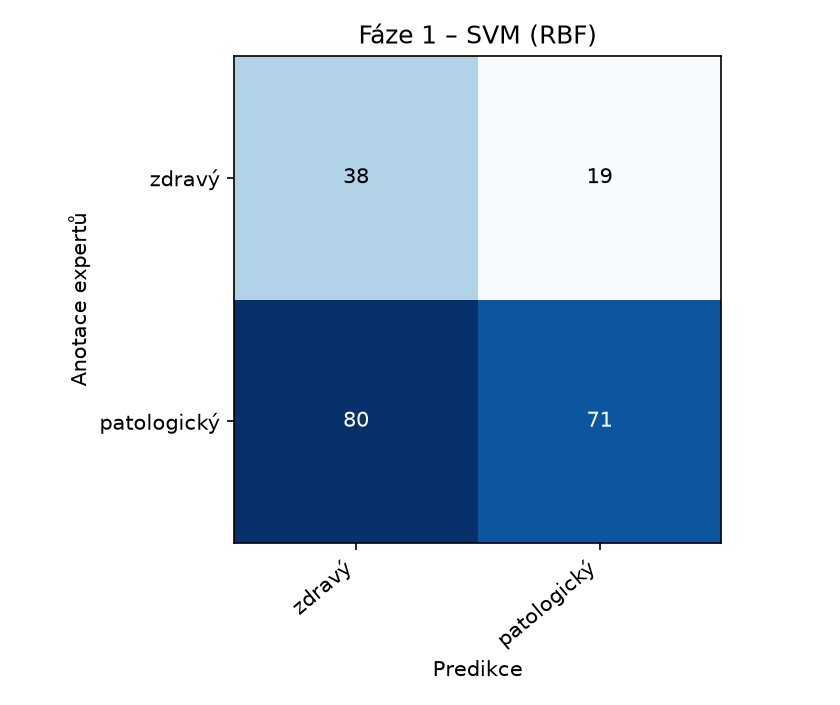
\includegraphics[width=\textwidth]{figures/faze1_matice_zamen.png}
  \caption{Fáze 1 (SVM)}
\end{subfigure}\hfill
\begin{subfigure}[t]{0.57\textwidth}
  \centering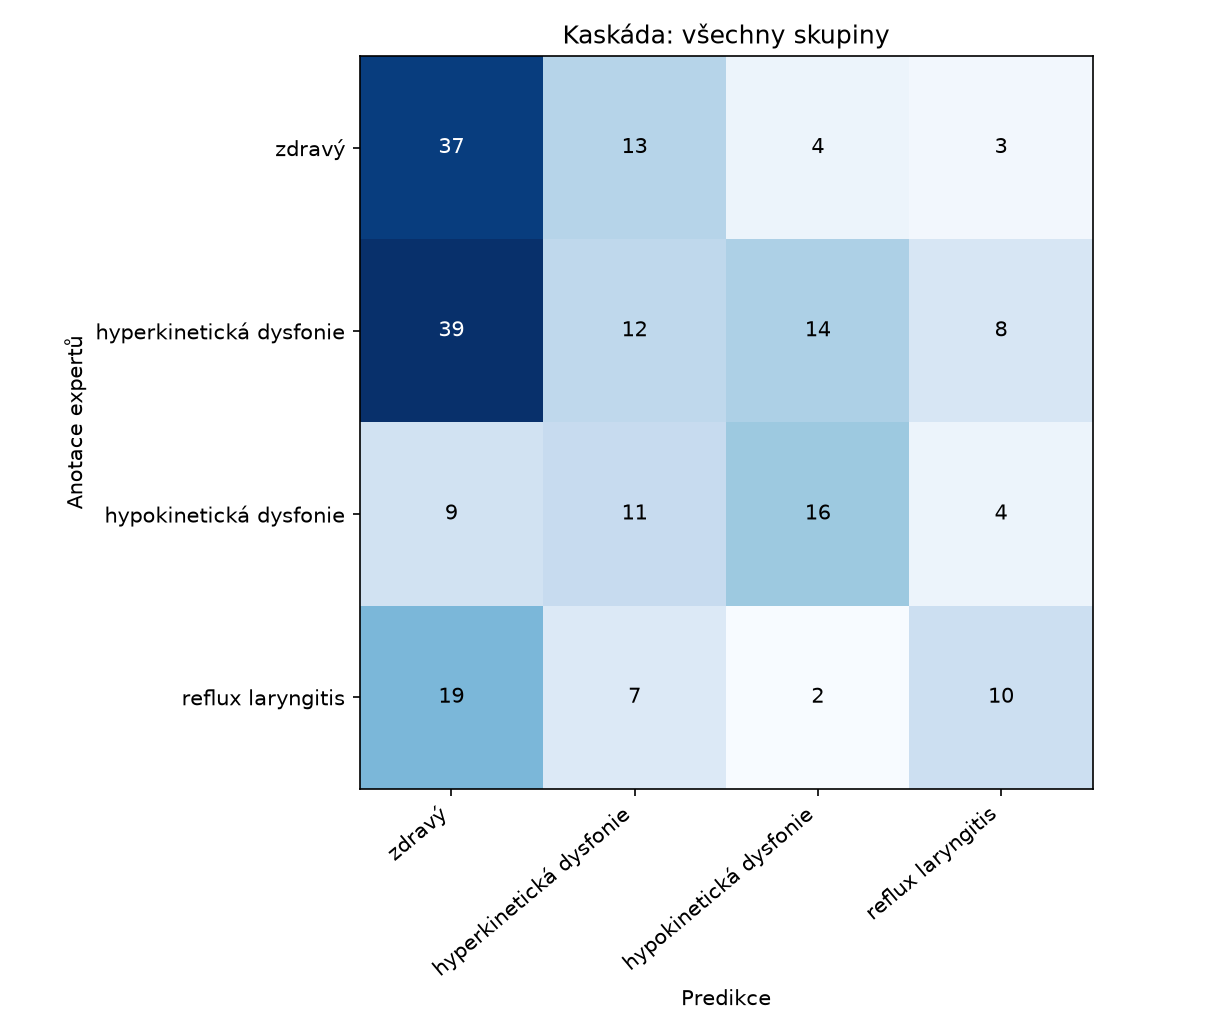
\includegraphics[width=\textwidth]{figures/kaskada_matice_zamen.png}
  \caption{Kaskáda (všechny skupiny)}
\end{subfigure}
\caption{Matice záměn, řádky jsou anotace expertů, sloupce predikce.}
\label{fig:matice}
\end{figure}

Největší chybou je, že 41 ze 73 hyperkinetických nahrávek se označí za zdravé. Reflux laryngitis se
nejčastěji zamění za zdravý hlas (18 ze 38). Hyperkinetická a hypokinetická dysfonie se zaměňují
navzájem (13 a 8 případů).

\subsection{Prostor příznaků}
V PCA (28,5~\% a 14,5~\% rozptylu, obr.~\ref{fig:pca}) se zdravé a patologické nahrávky i jednotlivé
poruchy prakticky zcela překrývají. Viditelné jsou jen odlehlé nahrávky vpravo (PC1 $>$ 8): 6 hypokinetických
a 4 hyperkinetické, což odpovídá nižšímu HNR a CPP hypokinetické dysfonie. Ani jednotlivé příznaky
skupiny dobře neoddělují (tab.~\ref{tab:auc}): nejlepší má AUC jen 0,69.

\begin{table}[H]
\centering\small
\caption{Nejlepší jednotlivé příznaky pro rozlišení zdravý $\times$ patologický (plocha pod ROC křivkou,
0,5 = náhoda). Úplná tabulka je v souboru \texttt{auc\_priznaku.csv}.}
\label{tab:auc}
\begin{tabular}{lrl}
\toprule
Příznak & AUC & Vyšší hodnota u\\
\midrule
plochost spektra           & 0,69 & patologických\\
směrodatná odchylka F0     & 0,64 & patologických\\
HNR (průměr)               & 0,64 & zdravých\\
jitter local               & 0,63 & patologických\\
shimmer local              & 0,61 & patologických\\
CPP (průměr)               & 0,61 & zdravých\\
\bottomrule
\end{tabular}
\end{table}

\begin{figure}[H]
\centering
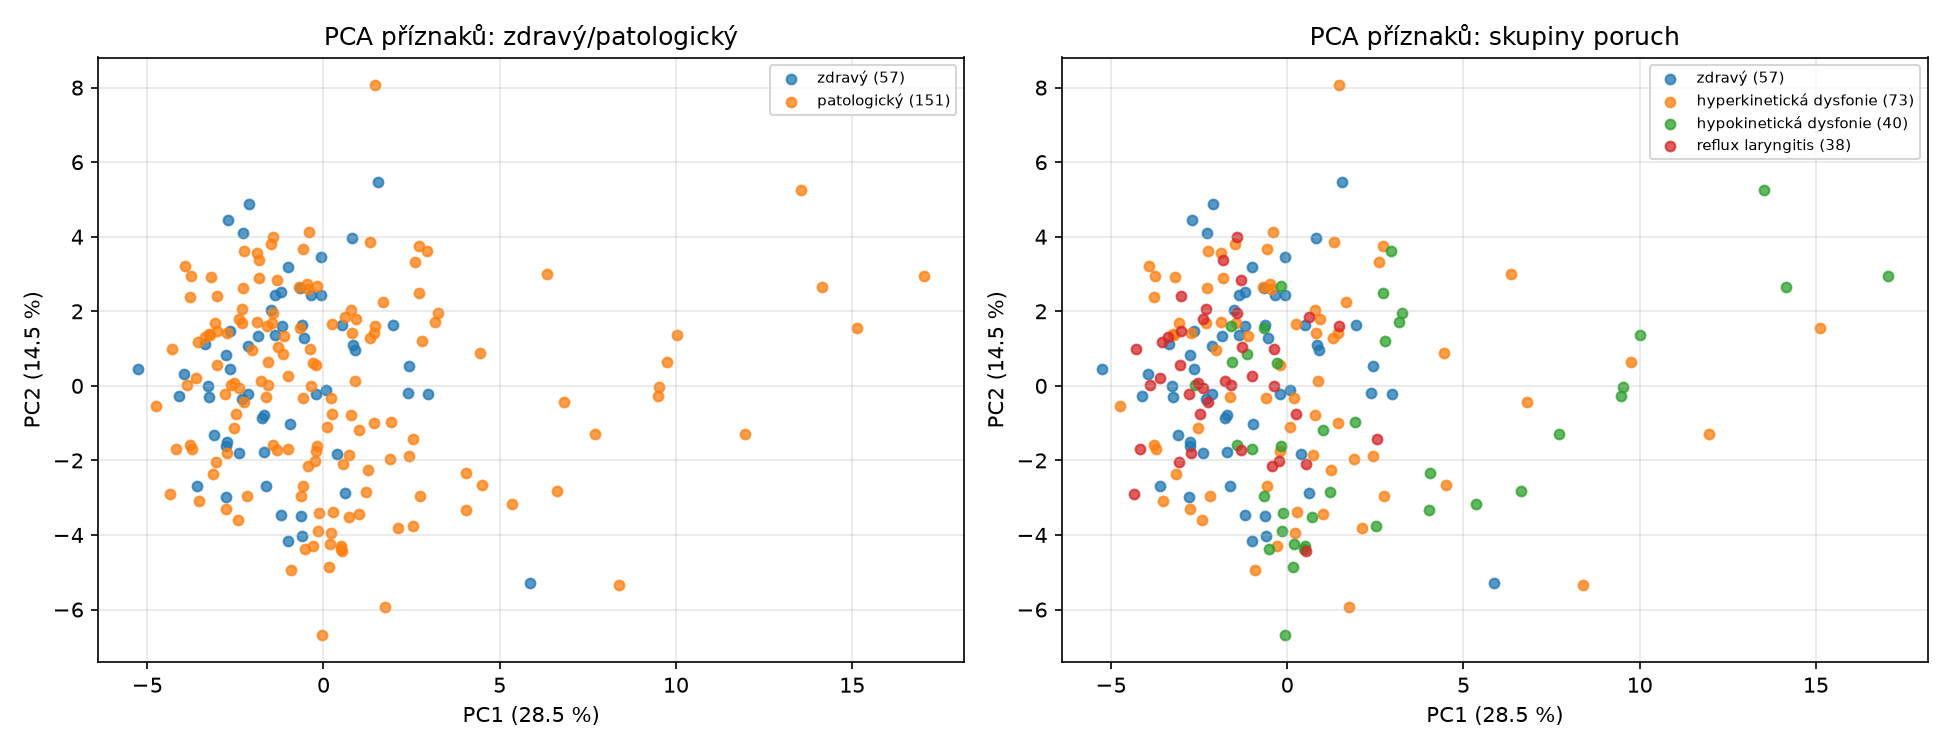
\includegraphics[width=\textwidth]{figures/pca.png}
\caption{PCA příznaků: vlevo zdravý a patologický hlas, vpravo skupiny poruch.}
\label{fig:pca}
\end{figure}

Nejlepší typ modelu (ze tří kandidátů) se vybíral na stejné vnější křížové validaci, kterou se hodnotí;
$k$ příznaků a hyperparametry klasifikátoru se ladí zanořeně na trénovací části každého foldu.

%==============================================================================
\section{Zhodnocení a závěr}
%==============================================================================
Příznaky odlišují zdravé a patologické hlasy v této databázi jen slabě, a proto je úspěšnost jen
mírně nad triviálními strategiemi.

\begin{itemize}
  \item \textbf{Výsledek.} Vyvážená přesnost fáze~1 je $57{,}2 \pm 2{,}2$~\% (triviálně 50~\%), fáze~2
        $52{,}7 \pm 1{,}6$~\% (triviálně 33~\%, přesnost $50{,}3$~\% proti triviálním 48,3~\%) a kaskáda
        dosahuje přesnosti 36,1~\% (triviálně 35,1~\%).
  \item \textbf{Příčiny.} Skupiny se silně překrývají: medián HNR je 14,8~dB u zdravých, 14,3~dB
        u hyperkinetické, 12,6~dB u hypokinetické a 14,9~dB u refluxu, s velkým rozptylem uvnitř
        skupin. Dalšími důvody jsou 45 příznaků na pouhých 208 nahrávek, nevyvážené třídy a řada
        mírně postižených hlasů.
  \item \textbf{Zaměňování.} Reflux laryngitis se nejčastěji zamění za zdravý hlas a hyperkinetická
        dysfonie se v kaskádě ztratí už ve fázi~1.
  \item \textbf{Omezení.} Výběr nejlepšího typu modelu probíhá na stejné vnější validaci (rozdíly
        mezi modely 2--3~p.b. jsou srovnatelné se směrodatnou odchylkou 1--3~p.b.); $k$ příznaků
        a hyperparametry klasifikátoru se ladí zanořeně. Použita je jen samohláska /a/.
  \item \textbf{Možná rozšíření.} Další samohlásky, formantové příznaky a větší počet pacientů.
\end{itemize}

%==============================================================================
\begin{thebibliography}{9}
\bibitem{physionet} Goldberger, A. L. et al.: PhysioBank, PhysioToolkit, and PhysioNet.
  \emph{Circulation}, 101(23):e215--e220, 2000.
\bibitem{voiced} Cesari, U. et al.: Voice Disorder Detection via an m-Health System: Design and
  Results of a Clinical Study to Evaluate Vox4Health. \emph{BioMed Research International},
  2018, 8193694. Databáze: \url{https://physionet.org/content/voiced/1.0.0/}.
\bibitem{boersma} Boersma, P.: Accurate short-term analysis of the fundamental frequency and the
  harmonics-to-noise ratio of a sampled sound. \emph{Proceedings of the Institute of Phonetic
  Sciences}, 17:97--110, 1993.
\bibitem{hillenbrand} Hillenbrand, J. et al.: Acoustic correlates of breathy vocal quality.
  \emph{Journal of Speech and Hearing Research}, 37:769--778, 1994.
\bibitem{davis} Davis, S. B., Mermelstein, P.: Comparison of parametric representations for
  monosyllabic word recognition in continuously spoken sentences. \emph{IEEE Transactions on
  Acoustics, Speech, and Signal Processing}, 28(4):357--366, 1980.
\bibitem{scipy} Virtanen, P. et al.: SciPy 1.0: fundamental algorithms for scientific computing
  in Python. \emph{Nature Methods}, 17:261--272, 2020.
\bibitem{sklearn} Pedregosa, F. et al.: Scikit-learn: Machine Learning in Python.
  \emph{Journal of Machine Learning Research}, 12:2825--2830, 2011.
\end{thebibliography}

\end{document}
